\documentclass[11pt]{article}

%%% These are some packages that are useful
\usepackage{circuitikz} %used for circuit diagrams
\usepackage{lastpage} %allows us to determine how many total pages there are
\usepackage{amsfonts, lipsum}
\usepackage{amsmath,amssymb, amscd,amsbsy, amsthm, enumerate}
\usepackage{mdframed, titlesec, setspace,verbatim, multicol}
\usepackage[top=1in, bottom=1in, left=1in, right=1in]{geometry} %sets the margins
\usepackage[unicode]{hyperref} %enhanced references
\usepackage{tikz, pgfplots, xcolor}
\usepackage{fancyhdr} %creates a fancy header for labeling document/name/date 
\usepackage{listings}
\usepackage{xcolor}
\usepackage{vwcol}  
\usepackage{enumitem}

%%% Page formatting
%\setlength{\headsep}{30pt}
\setlength{\parindent}{25pt}
\setlength{\textheight}{9in}

%%% Header and Footer Info
\pagestyle{fancy}
\fancyhead[L]{{\footnotesize \large PHY 482 - calculations}}
\fancyhead[C]{\footnotesize \today}
\fancyhead[R]{\footnotesize Name: Antonius Torode \& Eric Aboud}
\fancyfoot[L]{}
\fancyfoot[C]{}
\fancyfoot[R]{\thepage\ of \pageref{LastPage}}

%%Use these commands to clear the fancyhdr settings and horizontal header line.
%\fancyhf{} % sets both header and footer to nothing
%\renewcommand{\headrulewidth}{0pt}


%%% This defines the solution environment for you to write your solutions
\newenvironment{soln}
{\let\oldqedsymbol=\qedsymbol
	\renewcommand{\qedsymbol}{$ $}
	\begin{proof}[\bfseries\upshape \color{blue}Solution]\color{blue}}
	{\end{proof}
	\renewcommand{\qedsymbol}{\oldqedsymbol}}

\newenvironment{Deletion}
{\let\oldqedsymbol=\qedsymbol
	\renewcommand{\qedsymbol}{$ $}
	\begin{proof}[\bfseries\upshape \color{red}Deletion]\color{red}}
	{\end{proof}
	\renewcommand{\qedsymbol}{\oldqedsymbol}}


%%% Document Starts now
\begin{document} 

\begin{center}
	{\Large E\&M II - Project 2 Calculations.}
\end{center}

The \textbf{Zeeman effect} is an effect that comes about from putting an atom in a magnetic field. The magnetic field causes a magnetic moment to be produced and perturbs the energy levels of the atom causing spectral line shifts to appear when modeled or measured with spectroscopy. 

\section{Hydrogen Atom First Order Magnetic Field Energy Corrections}
To begin, the unperturbed wave functions of hydrogen is given by 
\begin{align}
H^{(0)} = \underbrace{\frac{\vec{p}^2}{2m}}_{\textrm{Kinetic term}}-\underbrace{\frac{\hbar c \alpha}{r}}_{\textrm{Potential term}}.
\end{align}
Consider the atom now in a magnetic field $\vec{B}$. The electrons spin will yield a magnetic moment $\vec{\mu}_S=\frac{-eg_s}{2m}\vec{S}$. The energy interaction of a single magnetic moment $\vec{\mu}$ with a fixed external magnetic field is given by $H^{\mu}= - \mu \cdot \vec{B}$ and so the Hamiltonian change due to this effect is $H_{S}^{(1)} =  -\mu_s \cdot \vec{B} = \frac{eg_s}{2m}\vec{S}\cdot \vec{B}$. There is also a correction due to the angular momentum of the electron. If we assume that the electron is moving in a circle, then this has a magnetic dipole $\mu_L = \frac{-e}{2m}\vec{L}$ and so there exists another correction to the Hamiltonian $H_L^{(1)} = -\mu_L \cdot\vec{B} = \frac{eg_L}{2m}\vec{L}\cdot \vec{B}$. Now, $g_s$ is a bi-products of the Dirac equation has a value of $g_s=s$. Combining these terms together give the total Zeeman effect to the Hamiltonian $H_{magnetic}^{(1)}$,
\begin{align}
H_{magnetic}^{(1)} \equiv H_{mag}^{(1)}= \frac{e}{2m}(\vec{L}+2\vec{S})\cdot \vec{B} = \frac{\mu_B}{\hbar}(\vec{L}+2\vec{S})\cdot \vec{B},
\end{align} 
where $\mu_B=\frac{e\hbar}{2m}$ is the Bohr magneton.

If we are just considering the changes that come about from the Zeeman effect, we can ignore other Hamiltonian perturbations such as the fine structure and hyperfine structure interactions. Assume that $\vec{B} \equiv B\hat{z}$ then the Hamiltonian will only contain z components after performing the dot product giving $H_{mag}^{(1)} = \frac{\mu_B}{\hbar}(L_z+2S_z)B$. Now, $\vec{J}=\vec{L}+\vec{S} \implies L_z = J_z-S_z$ and so
$H_{mag}^{(1)} = \frac{\mu_B}{\hbar}(J_z+S_z)B$. From perturbation theory we can solve for the first order energy corrections to this using
\begin{align}
E_{n}^{(1)} &= \langle n j m_j \ell s| H_{mag}^{(1)}|n j m_j \ell s \rangle \nonumber\\
&= \frac{\mu_BB}{\hbar}\langle n j m_j \ell s| (J_z+S_z)|n j m_j \ell s \rangle \nonumber\\
&= \frac{\mu_BB}{\hbar}\left(\hbar m_j+\langle n j m_j \ell s| S_z|n j m_j \ell s \rangle \right). \label{<njmls|S_z|nlmls>}
\end{align}
We can determine $S_z$ by projecting $\vec{S}$ onto $\vec{J}$ which gives $\vec{S} = \frac{\vec{J}\cdot\vec{S}}{\vec{J}^2}\vec{J}$ and then using the substitution that 
\begin{align}
\vec{J}\cdot \vec{S} = (\vec{L}+\vec{S})\cdot \vec{S} = \vec{L}\cdot\vec{S}+\vec{S}^2 = \frac{1}{2}(\vec{J^2}-\vec{L^2}-\vec{S}^2)+\vec{S^2} = \frac{1}{2}(\vec{J^2}-\vec{L^2}+\vec{S}^2).
\end{align}
This, we have
\begin{align}
S_z = \frac{(\vec{J^2}-\vec{L^2}+\vec{S}^2)}{2\vec{J}^2}J_z,
\end{align}
and so the undetermined matrix element in (\ref{<njmls|S_z|nlmls>}) becomes 
\begin{align}
\langle n j m_j \ell s| S_z|n j m_j \ell s \rangle &= \langle n j m_j \ell s| \frac{(\vec{J^2}-\vec{L^2}+\vec{S}^2)}{2\vec{J}^2}J_z|n j m_j \ell s \rangle \nonumber \\
&= m_j \hbar \frac{j(j+1)-\ell(\ell+1)+s(s+1)}{2j(j+1)}.
\end{align}
Plugging this back into (\ref{<njmls|S_z|nlmls>}) gives a general result
\begin{align}
\boxed{E_{n}^{(1)} = \mu_BBm_j\left[1+\frac{j(j+1)-\ell(\ell+1)+s(s+1)}{2j(j+1)}\right] = \mu_BBm_jg_L}, \label{E_{n}^{(1)}}
\end{align}
where $g_L$ is the Land\'{e} g factor
\begin{align}
g_L = 1+\frac{j(j+1)-\ell(\ell+1)+s(s+1)}{2j(j+1)}.
\end{align}
Note that for the hydrogen atom such as we have, the spin $s=\frac{1}{2}$ so we can further simplify this to 
\begin{align}
E_{n}^{(1)} = \mu_BBm_j\left[1+\frac{j(j+1)-\ell(\ell+1)+\frac{3}{4} }{2j(j+1)} \right].
\end{align}

\subsection{Example Energy Correction: $2P_{3/2}$}
This result in (\ref{E_{n}^{(1)}}) can be used for an explicit state of the hydrogen atom. For example, consider the $2P_{3/2}$ state. This has $n=2$, $\ell =1$, $s=\frac{1}{2}$, and $j=\frac{3}{2}$. The $m_j$ values can thus be determined by the set $m_j = \{m_j=j+n|-j \geq m_j \geq j \textrm{ and } n \in \mathbb{Z}\} = \{-\frac{3}{2},-\frac{1}{2}, \frac{1}{2}, \frac{3}{2} \}$, which tells us there will be 4 different energy splits for this state. Using these values gives us a $g_L=\frac{4}{3}$ and so our energy splits are
\begin{align}
E_{2P_{3/2}}^{(1)} = \begin{cases}
\frac{\mu_BB}{2} & \textrm{for }m_j = \frac{3}{2}\\ 
\frac{2\mu_BB}{3} & \textrm{for }m_j = \frac{1}{2} \\
-\frac{2\mu_BB}{3}& \textrm{for }m_j = -\frac{1}{2} \\
-\frac{\mu_BB}{2} & \textrm{for }m_j = -\frac{3}{2}
\end{cases}  
\end{align}

\section{Linearly Changing Magnetic Field}

Consider Maxwell's Equations, which are the system of partial differential equations describing classical electromagnetism. $\vec{P}$ is the polarization field, $\vec{D}$ is the electric displacement field, $\rho$ is the charge density, $\vec{E}$ is the electric field, $\vec{B}$ is the magnetic field, and $\vec{J}$ is the current density. In the MKS system of units (where $\epsilon_0$ is the permittivity of free space and $\mu_0$ is the permeability of free space), the equations are written 
\begin{multicols}{2}
	\noindent
	\begin{align}
	\nabla \cdot \vec{E} &= \frac{\rho}{\epsilon_0} \label{nabla cdot E}\\
	\nabla \times \vec{E} &= -\frac{\partial \vec{B}}{\partial t} \label{nabla times E}
	\end{align}
	\begin{align}
	\nabla \cdot \vec{B} &= 0  \label{nabla cdot vecB}\\
	\nabla \times \vec{B} &= \mu_0\vec{J}+\epsilon_0\mu_0\frac{\partial \vec{E}}{\partial t} \label{nabla times vecB}
	\end{align}
\end{multicols}
It may seem reasonable to look at the Zeeman effect with regards to a linear magnetic field since that would be a simple case. However should we model this as a linear $\vec{B}$ with regard to position or linear $\vec{B}$ with regard to time? If we allow $\vec{B}_{linear, z} \equiv B z \hat{z}$, then we can see there is a violation of (\ref{nabla cdot vecB}). This can be easily seen as $\nabla \cdot B z \hat{z} = B \neq 0$ for any $b\neq 0$. This is an impossible magnetic field. 

Consider $\vec{B} = Bt \hat{z}$. The divergence is zero since it has no spacial dependence which satisfies (\ref{nabla cdot vecB}). Similarly, the curl is zero for the same reason. If we assume we are within a vacuum (other than our single hydrogen atom we are modeling), then by (\ref{nabla times vecB}), we have $\frac{\partial \vec{E}}{\partial t} = 0$, which implies the electric field is a constant throughout time. By (\ref{nabla times E}), the electric field must satisfy $\nabla \times \vec{E} = -B \hat{z}$. If we take the curl of both sides of this we get
\begin{align}
\nabla \times(\nabla \times \vec{E}) = \nabla (\nabla \cdot \vec{E})- \nabla^2 \vec{E} = -\nabla \times B \hat{z} =0.
\end{align}
Using our assumption of a vacuum and (\ref{nabla cdot E}), this becomes 
\begin{align}
 \nabla^2 \vec{E} =  0 \implies \frac{\partial^2 E_x}{\partial x^2}+\frac{\partial^2 E_y}{\partial y^2}+\frac{\partial^2 E_z}{\partial z^2}=0 \label{del^2 E=0}
\end{align}

Consider a one dimensionally changing electric field with spacial dependence and no time dependence. This could potentially be produced in a lab so it is a good example. We can see a trivial solution to this would be $\vec{E}_1 = (ax+by+cz) \hat{x}$, where $a,b,c$ are some constants. By (\ref{nabla times E}), we know 
\begin{align}
c \hat{y}-b \hat{z} = -B \hat{z} \implies b \equiv B \textrm{ and } c \equiv 0 \implies \vec{E}_1 = B y\hat{x}. \label{c haty-b hatz}.
\end{align}
We can see that $a$ has no requirements and so it can be arbitrary. For simplicity we can make $a=0$. In fact, upon a closer look, $a=0$ is the only possible choice in order for (\ref{nabla cdot E}) to remain satisfied. So thus from out magnetic field $\vec{B} = Bt\hat{z}$, we require that there also be an electric field $\vec{E}_1=By \hat{x}$ in order for Maxwell's equations to be satisfied. Let us double check quickly. 
\begin{align}
&\textrm{(\ref{nabla cdot E}): }\nabla \cdot \vec{E}_1 = \nabla \cdot By \hat{x} = \frac{\partial}{\partial x} By = 0 \hspace{1cm} \checkmark \\
&\textrm{(\ref{nabla cdot vecB}): } \nabla \cdot \vec{B} = \nabla \cdot Bt \hat{z} = \frac{\partial}{\partial z} Bt = 0 \hspace{1cm} \checkmark \\
&\textrm{(\ref{nabla times E}): } \nabla \times \vec{E}_1 = \nabla \times B y \hat{x} = -B \hat{z} = -\frac{\partial \vec{B}}{\partial t}   \hspace{1cm} \checkmark \\
&\textrm{(\ref{nabla times vecB}): } \nabla \times \vec{B} = \nabla \times Bt\hat{z} = 0 = \mu\epsilon_0\frac{\partial \vec{E}}{\partial t}\hspace{1cm} \checkmark 
\end{align}
Does this solution make sense physically? We have a magnetic field changing uniformly through time and it creates an electric field that is linearly increasing in y space in the $\hat{x}$ direction. By analogy we can also find another solution to $\vec{E}$ by assuming $\vec{E}_2 = (ax+by+cz)\hat{y}$ and then by a method analogous to (\ref{c haty-b hatz}), we get $\vec{E}_2 = -Bx\hat{y}$. And so by superposition we can also have a solution
\begin{align}
\vec{E}_{1+2} = B(y \hat{x}-x\hat{y}).
\end{align}
If we plot this using Mathematica we can see that it's a radial function around the z axis where our magnetic field is changing, which makes sense for it to be radially dependent. However, if we notice, it is increasing with r, which means it is divergent and thus does not make sense physically (see Figure 1).

\begin{center}
	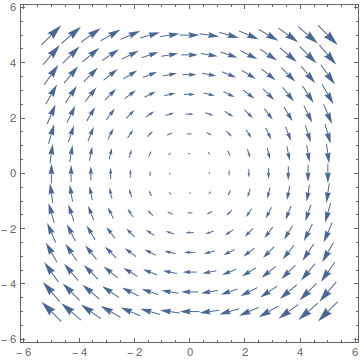
\includegraphics[]{E1plus2.png}
	
	{\footnotesize \textbf{Figure 1.} A plot of $\vec{E}_{1+2}$ using B=1 in the x-y plane.}
\end{center}

From this example we can see that we cannot just guess a solution to (\ref{del^2 E=0}). Instead we can find a general solution and impose boundary conditions in order to find an electric field that will physically work and make sense in our situation.

\begin{center}
	\textbf{Hypothesis.} I suspect the possible inconsistency above comes about from assuming we are in a vacuum if not a mistake in a calculation somewhere. I will attempt to look into this further if I have any free time after finishing the E \& M homework assignment and exam prep for tomorrow.
\end{center}


\section{Changing Electric Field}

\begin{Deletion}
Consider a linearly changing electric field with position, $\vec{E} = E y\hat{z}$. This is an electric field moving along the $\hat{z}$ direction that is linearly increasing with $y$. We can use (\ref{nabla times E}) to determine a potential magnetic field that will go along with this electric field. This gives 
\begin{align}
\vec{B} = -\int (\nabla \times \vec{E}) dt 
= -\int (\nabla \times Ey \hat{z}) dt 
= -\int \begin{vmatrix}
\hat{x} & \hat{y} & \hat{z} \\
\frac{\partial}{\partial x} & \frac{\partial}{\partial y} & \frac{\partial}{\partial z} \\
0 & 0 & Ey
\end{vmatrix} dt 
= -\int E dt =-E\Delta t.
\end{align}
This verifies the previous calculation. Duh.
\end{Deletion}

Consider a magnetic field that is strong and decreases as distance falls off. That is something such as $\vec{E} = \frac{E_0}{y}$.


\begin{thebibliography}{9}
	\bibitem{brain} Our brains.
\end{thebibliography}
%%%%%%%%%%%%%%%%%%%%%%%%%%%%%%%%%%%%%%%%%%%%%%%%%%%%%%%%%%%%%%%%%%%%%%%%%%%%%%%%%%%%%%%%%%%

%%%%%%%%%%%%%%%%%%%%%%%%%%%%%%%%%%%%%%%%%%%%%%%%%%%%%%%%%%%%%%%%%%%%%%%%%%%%%%%%%%%%%%%%%%%
\end{document}





















